%!TEX root = ../Main.tex
\section{Benchmarks}
\label{s:Benchmarks}
%!TEX root = ../Main.tex

\begin{figure}

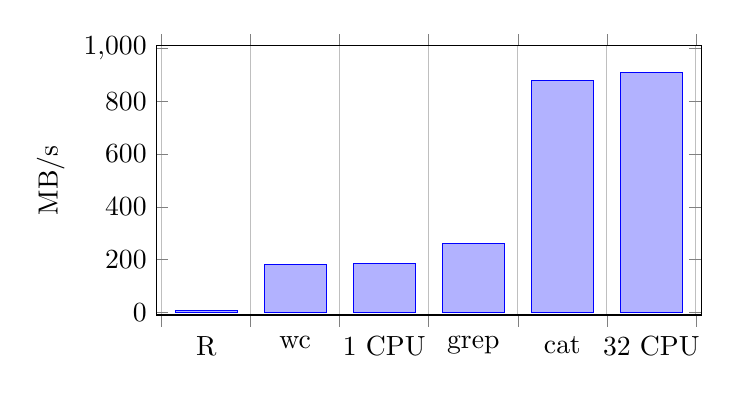
\begin{tikzpicture}
\begin{axis}[
	ylabel=MB/s,
  ymin=0, ymax=1000,
	enlargelimits=0.01,
	ybar interval=0.7,
  symbolic x coords={R, wc, 1 CPU, grep, cat, 32 CPU, end},
  width=8.5cm, height=5cm,
]
\addplot coordinates {(R,6.0) (wc,182.6) (1 CPU,186.6) (grep,261) (cat,878) (32 CPU,908) (end,0) };
% \addplot coordinates {(R,6.0) (wc,182.6) (CPU1,186.6) (grep,261) (wc -l,852) (cat,878) (Run 372,908) (Run 1,1029) (end,0) };

% \legend{MB/s}

\end{axis}
\end{tikzpicture}

\caption{Throughput comparisons of Icicle (1 CPU and 32 CPU) against existing R code and standard Unix utilities; higher is faster.}
\label{fig:bench:other}
\end{figure}



At Ambiata, we are currently using Icicle in production over medium-sized datasets that fit on a single disk.
These initial results have been very promising, and we are currently implementing distribution across multiple machines to handle datasets that are tens of terabytes compressed, and do not fit on a single disk.
Incremental computation is even more important for this distributed case, as we can avoid copying terabytes of data over the network.

We evaluated Icicle by replacing an R script which ran weekly in production.
This R script works over around three hundred gigabytes of PSV data.
It computes twelve queries over each of the thirty-one input tables, computing 372 queries in total.

The R script for this takes fifteen hours to run and is 3,566 lines of code.
In contrast, our Icicle queries take seven minutes to run, and the dictionary describing the queries is 191 lines of code.

The table in figure~\ref{fig:bench:other} shows the throughput in megabytes per second.
We compared the throughput of several programs over the same 317GB dataset:
\begin{itemize}
\item our original R implementation (R);
\item Icicle running single-threaded (1 CPU);
\item Icicle running on multiple processors (32 CPU);
\item finding empty lines with @grep "^$"@;
\item counting characters, words and lines with @wc@;
\item reading and throwing away the results with @cat > /dev/null@.
\end{itemize}

We ran all of the Unix utilities with unicode disabled using @LANG=C LC_COLLATE@ for maximum performance.
The computer we used for most of these was an Amazon EC2 @c3.8xlarge@ with 32 CPUs, 60GB of RAM, and striped, RAIDed SSD storage.
The R code requires an @i2.8xlarge@ with 244GB of memory, but we were unable to perform our other benchmarks on such a large machine.
Icicle significantly outperformed R, and the single-threaded version was on par with @wc@, while only a little slower than @grep@.
This is despite doing conceptually more work than @wc@ and @grep@.
By using multiple processors, we were able to scale up to perform as well as @cat@, approaching the disk speed.
The R code is single threaded and would require at least 150 processors to reach similar speeds, assuming perfect scaling.
These results give us confidence that our distributed implementation will be performant as well as scalable~\cite{mcsherry2015scalability}.

%!TEX root = ../Main.tex

\begin{figure}

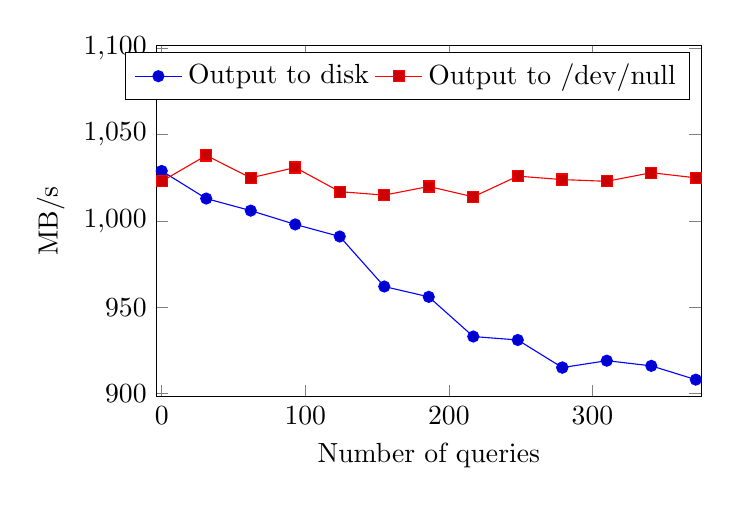
\begin{tikzpicture}
\begin{axis}[
	x tick label style={/pgf/number format/1000 sep=},
	ylabel=MB/s,
  ymin=900, ymax=1100,
%  xmax=372,
  xlabel=Number of queries,
	enlargelimits=0.01,
	legend style={legend columns=-1},
  width=8.5cm, height=6.05cm,
%	legend style={at={(0.5,-0.1)},anchor=north,legend columns=-1},
%	ybar interval=0.7,
]

% bench/raw.txt
% Running with fewer queries
% \addplot coordinates {(0,1025.5) (1,1029.6) (48,978) (96,941) (144,943) (192,936) (240,904) (276,895.5) (324,881) (372,846.2) };

% bench/raw.txt
% Running with fewer queries, better distribution
% \addplot coordinates { (0,1029) (31,1013) (62,1006) (93,998) (124,991) (155,941) (186,956) (217,933) (248,931) (279,915) (279,915) (310,919) (341,916) (372,908) };

%% APPLY LOPASS
\addplot coordinates { (0,1029) (31,1013) (62,1006) (93,998) (124,991) (155,962) (186,956) (217,933) (248,931) (279,915) (279,915) (310,919) (341,916) (372,908) };


% Fusion, no output
% \addplot coordinates { (0,1001) (31,1038) (62,1025) (93,1031) (124,1006) (155,1015) (186,1020) (217,997) (248,1026) (279,1024) (310,1009) (341,1038) (372,1025) };

%% APPLY LOPASS
\addplot coordinates { (0,1023) (31,1038) (62,1025) (93,1031) (124,1017) (155,1015) (186,1020) (217,1014) (248,1026) (279,1024) (310,1023) (341,1028) (372,1025) };

% No fusion, no output
% \addplot coordinates { (0,987) (31,1037) (62,1024) (93,1002) (124,1037) (155,1024) (186,1004) (217,1040) (248,1023) (279,998) (310,1018) (341,1013) (372,1003) };

\legend{Output to disk, Output to /dev/null};

\end{axis}
\end{tikzpicture}


\caption{Decrease in read throughput as queries are added, comparing writing the output to disk and writing to /dev/null.}
\label{fig:bench:queries}
\end{figure}


% \begin{figure}
% \begin{tikzpicture}
% \begin{axis}[
% 	x tick label style={/pgf/number format/1000 sep=},
% 	ylabel=MB/s,
%   ymin=0, ymax=1200,
%   xlabel=Number of threads,
% 	enlargelimits=0.01,
% 	legend style={legend columns=-1},
% ]
% \addplot coordinates { (1,163) (2,335) (3,442) (4,532) (5,578) (6,615) (7,633) (8,628) (9,631) (10,626) (11,637) (12,643) (13,658) (14,795) (15,781) (16,798) (17,840) (18,864) (19,862) (20,867) (21,847) (22,877) (23,876) (24,884) (25,862) };
% \end{axis}
% \end{tikzpicture}
% \caption{Scaling as threads are added}
% \label{fig:bench:scaling}
% \end{figure}




Figure~\ref{fig:bench:queries} shows how Icicle scales in throughput as more queries are added.
We ran two versions with each number of queries; one version writing output to disk, and the other throwing away the result to @/dev/null@ rather than spending time writing.
The graph shows the disk version decreasing roughly linearly in the number of queries, while the version ignoring the output stays constant.
This suggests that the output code is the bottleneck, which is unsurprising given the output format is text-based PSV.
The upshot of this is that the time spent computing the queries appears constant as hundreds of queries are added, which suggests that many more queries can be handled.

